\documentclass[12pt,a4paper]{report}
%\documentclass[12pt, twoside,openright]{report}
\usepackage[]{graphicx}
%\usepackage{fontspec}
%\setmainfont{Code2000}
%\usepackage{,epsfig}
\usepackage[centertags]{amsmath}
\usepackage{epstopdf,amsfonts,epsfig,cite,array,multirow,graphicx,amsmath,amsthm,ltablex,tabularx,setspace,arydshln,amssymb,multirow,enumerate, mathtools}
%%%%%%% Inline listing package
%\usepackage[inline]{enumitem}
\DeclareMathOperator{\arccot}{arccot}
\DeclareMathOperator{\sinc}{sinc}
%\usepackage{marvosym}
%\usepackage{moderncvcompatibility}
\usepackage{geometry}
\geometry{tmargin=20mm,bmargin=20mm,lmargin=30mm,rmargin=25mm}
%\usepackage[cmex10]{amsmath}
\newcommand{\matr}[1]{\mathbf{#1}}

%%%%%%%%%%%% Run this package final time or if any error %%%%%%%%%
%\usepackage{fancyhdr}
\usepackage[titletoc]{appendix}
\usepackage[usenames,dvipsnames]{xcolor}
\usepackage{graphics}
\usepackage{cite}
\usepackage{amsmath}
\usepackage{amssymb}
\usepackage{amsfonts}
\usepackage{tikz}
\usepackage{setspace}
\usepackage{color}
\usepackage{relsize}
\usepackage{bigints}
\usetikzlibrary{shapes,arrows,fit,calc,positioning}
\usetikzlibrary{decorations.shapes}
\definecolor{colorgreen}{rgb}{0.2,0.5,0.3}
\definecolor{colorblue}{rgb}{0,0,0}
\usetikzlibrary{decorations.pathmorphing}
\usepackage{subfigure}
%\usepackage{hyperref}
\usepackage{ellipsis}
\usetikzlibrary{calc}
\usetikzlibrary{decorations.pathreplacing,decorations.markings,shapes.geometric}
\tikzset{naming/.style={align=center,font=\small}}
\tikzset{antenna/.style={colorblue, thick,insert path={-- coordinate (ant#1) ++(0,0.2) -- +(135:0.2) + (0,0) -- +(45:0.2)}}}
\tikzset{station/.style={naming,draw,shape=dart, thick,colorblue,shape border rotate=90, minimum width=15mm, minimum height=15mm,outer sep=0pt,inner sep=3pt}}
\tikzset{stationnew/.style={naming,draw,shape=dart, thick,colorblue,shape border rotate=90, minimum width=20mm, minimum height=20mm,outer sep=0pt,inner sep=3pt}}
%\tikzset{mobile/.style={naming,draw,shape=rectangle,minimum width=15mm,minimum height=7.5mm, outer sep=0pt,inner sep=3pt}}
\tikzset{mobile/.style={naming,draw,shape=rectangle,fill=olive!40,minimum width=3mm,minimum height=3mm, outer sep=0pt,inner sep=3pt}}
\tikzset{radiation/.style={{decorate,decoration={expanding waves,angle=90,segment length=4pt}}}}
\tikzset{
  double arrow/.style args={#1 colored by #2 and #3}{
    -stealth,line width=#1,#2, % first arrow
    postaction={draw,-stealth,#3,line width=(#1)/3,
                shorten <=(#1)/3,shorten >=2*(#1)/3}, % second arrow
  }
}

\tikzset{
  double dasharrow/.style args={#1 colored by #2 and #3}{
    -stealth,dashed,line width=#1,#2, % first arrow
    postaction={draw,-stealth,#3,line width=(#1)/3,
                shorten <=(#1)/3,shorten >=2*(#1)/3}, % second arrow
  }
}



\newcommand{\UE}[1]{%
\begin{tikzpicture}[every node/.append style={rectangle,minimum width=0pt}]
\node[mobile] (box) {#1};

\draw ([xshift=.25cm] box.south west)
      ([xshift=-.25cm]box.south east);

%\fill ([xshift=.25cm] box.south west) circle (1pt)
%      ([xshift=-.25cm]box.south east) circle (1pt);

\draw (box.north) [antenna=1];
\end{tikzpicture}
}



\newcommand{\BS}[1]{%
\begin{tikzpicture}
\node[station] (base) {#1};

%\draw[line join=bevel] (base.110) -- (base.70) -- (base.north west) -- (base.north east) -- cycle;
\draw[line join=bevel,colorblue] (base.100) -- (base.80) -- (base.110) -- (base.70) -- (base.north west) -- (base.north east);
\draw[line join=bevel,colorblue] (base.100) -- (base.70) (base.110) -- (base.north east);

% original yshift=.8pt
\draw[line cap=rect] ([yshift=0pt]base.north) [antenna=1];
\end{tikzpicture}
}

\newcommand{\BSnew}[1]{
	\begin{tikzpicture}[scale=2.0]
	\node[stationnew] (base) {#1};
	
	\draw[line join=bevel] (base.110) -- (base.70) -- (base.north west) -- (base.north east) -- cycle;
	\draw[line join=bevel,colorblue] (base.100) -- (base.80) -- (base.110) -- (base.70) -- (base.north west) -- (base.north east);
	\draw[line join=bevel,colorblue] (base.100) -- (base.70) (base.110) -- (base.north east);
	
	% original yshift=.8pt
	\draw[line cap=rect] ([yshift=0pt]base.north) [antenna=1];
	\end{tikzpicture}
}

\newcommand{\RELAY}[1]{%
\begin{tikzpicture}[scale=0.2]
%\node[] (naming) {#1};
            \draw[thick,colorblue] (0,0) -- (1,4);% left line
            \draw[thick,colorblue] (3,0) -- (2,4);% right line
            \draw[semithick,colorblue] (0,0) arc (180:0:1.5 and -0.5) node[above, midway]{#1};
            \node[inner sep=4pt,colorblue] (circ) at (1.5,5.5) {};
            \draw[semithick,colorblue] (1.5,5.5) circle(8pt);
            \draw[semithick,colorblue] (1.5,5.5cm-8pt) -- (1.5,4);
            \draw[semithick,colorblue] (1.5,4) ellipse (0.5 and 0.166);
            \draw[semithick,radiation,decoration={angle=45}] (1.5cm+8pt,5.5) -- +(0:2);
            \draw[semithick,radiation,decoration={angle=45}] (1.5cm-8pt,5.5) -- +(180:2);
            %\fill[color = Aquamarine!80](0,0)--(1,4) -- (2,4)--(3,0)--cycle ;


\end{tikzpicture}
}

\newcommand{\RELAYnew}[1]{%
	\begin{tikzpicture}[scale=0.25]
	%\node[] (naming) {#1};
	\draw[thick,colorblue] (0,0) -- (1,4);% left line
	\draw[thick,colorblue] (3,0) -- (2,4);% right line
	\draw[semithick,colorblue] (0,0) arc (180:0:1.5 and -0.5) node[above, midway]{#1};
	\node[inner sep=4pt,colorblue] (circ) at (1.5,5.5) {};
	\draw[semithick,colorblue] (1.5,5.5) circle(8pt);
	\draw[semithick,colorblue] (1.5,5.5cm-8pt) -- (1.5,4);
	\draw[semithick,colorblue] (1.5,4) ellipse (0.5 and 0.166);
	\draw[semithick,radiation,decoration={angle=45}] (1.5cm+8pt,5.5) -- +(0:2);
	\draw[semithick,radiation,decoration={angle=45}] (1.5cm-8pt,5.5) -- +(180:2);
	%\fill[color = Aquamarine!80](0,0)--(1,4) -- (2,4)--(3,0)--cycle ;
	
	
	\end{tikzpicture}
}

\newcommand{\MBS}[1]{%
\begin{tikzpicture}
\node[stationnew] (base) {#1};

%\draw[line join=bevel] (base.110) -- (base.70) -- (base.north west) -- (base.north east) -- cycle;
\draw[line join=bevel,colorblue] (base.100) -- (base.80) -- (base.110) -- (base.70) -- (base.north west) -- (base.north east);
\draw[line join=bevel,colorblue] (base.100) -- (base.70) (base.110) -- (base.north east);

% original yshift=.8pt
%\draw[line cap=rect] ([xshift=.5cm,yshift=.3pt] base.north) [antenna=1];
%\draw[line cap=rect] ([yshift=.3pt]ant1 |- base.north) -- node[above,shape=rectangle,inner ysep=+.3333em]{\dots} ([xshift=-.5cm,yshift=.3pt]base.north) [antenna=2];
\draw[line cap=rect] ([xshift=-.1768cm,yshift=.6pt]base.north -| base.right tail) [antenna=1];

\draw[line cap=rect] ([yshift=.6pt]ant1 |- base.north) -- node[above,shape=rectangle,inner ysep=+.3333em]{\dots} ([xshift=.1768cm,yshift=.6pt]base.north -| base.left tail) [antenna=2];

\draw[line cap=rect] ([yshift=.6pt]ant1 |- base.north) -- node[above,shape=rectangle,inner ysep=+.3333em,]{\dots} ([xshift=.1768cm,yshift=.6pt]base.north -| base.left tail) [antenna=3];
%\draw[line cap=rect] ([yshift=.3pt]ant1 |- base.north) -- ([xshift=-.5cm,yshift=.3pt]base.north) [antenna=2];
%\node at ($(ant1)!0.5!(ant2)$) {\dots};
\end{tikzpicture}
}


\newcommand{\MOBILE}[1]{%
\begin{tikzpicture}[scale=0.25]
\begin{scope}[line join=round,looseness=0.25, line cap=round]
\begin{scope}
\clip [preaction={left color=blue!10, right color=blue!30}]
  (1/2,-1) to [bend left] (0,10)
  to [bend left] ++(1,1) -- ++(0,2)
  arc (180:0:3/4 and 1/2) -- ++(0,-2)
  to [bend left]  ++(5,-2) coordinate (A) to [bend left] ++(-1/2,-11)
  to [bend left] ++(-1,-1) to [bend left] cycle;
%
\path [left color=blue!30, right color=blue!50]
  (A) to [bend left] ++(0,-11) to[bend left] ++(-3/2,-2)
  -- ++(0,12);
%
\path [fill=blue!20, draw=white, line width=0.25cm]
  (0,10) to [bend left] ++(1,1) -- ++(0,2)
  arc (180:0:3/4 and 1/2) -- ++(0,-2)
  to [bend left]  (A) to [bend left] ++(-3/2,-5/4)
  to [bend right] cycle;
%
\draw [line width=0.25cm, fill=white]
  (9/8,21/2) arc (180:360:5/8 and 3/8) --
  ++(0,2.5) arc (0:180:5/8 and 3/8) -- cycle;
%
\draw [line width=0.25cm, fill=white]
  (9/8,13) arc (180:360:5/8 and 3/8);
%
\fill [white, shift=(225:0.5)]
  (1,17/2) to [bend left] ++(4,-7/4)
  to [bend left] ++(0,-7/2) to [bend left] ++(-4, 6/4)
  to [bend left] cycle;
%
\fill [black, shift=(225:0.25)]
  (1,17/2) to [bend left] ++(4,-7/4)
  to [bend left] ++(0,-7/2) to [bend left] ++(-4, 6/4)
  to [bend left] cycle;
%
\shade [inner color=white, outer color=cyan!20]
  (1,17/2) to [bend left] ++(4,-7/4)
  to [bend left] ++(0,-7/2) to [bend left] ++(-4, 6/4)
  to [bend left] cycle;
\draw [line width=0.25cm, shorten <=-0.5cm, shorten >=-0.5cm]
  (1,17/2) to [bend left] ++(4,-7/4)
  to [bend left] ++(0,-7/2);
%
\foreach \i in {1,2,3}
  \foreach \j in {1,2,3}
     \draw [line width=0.125cm, top color=gray,
       bottom color=white, yslant=-3/8, rounded corners=1cm/8]
         (\i*3/2-1/2,-\j+4) rectangle ++(1,3/4);
%
\draw [line width=0.125cm, top color=gray, bottom color=white, yslant=-3/8]
  (3,0) ellipse [x radius=1/2, y radius=1/3];
%
\draw [line width=0.125cm, top color=gray, bottom color=white, yslant=-3/8]
  (3,19/2) ellipse [x radius=1, y radius=1/4];
\end{scope}
\draw [line width=0.5cm]
  (1/2,-1) to [bend left] (0,10)
  to [bend left] ++(1,1) -- ++(0,2)
  arc (180:0:3/4 and 1/2) -- ++(0,-2)
  to [bend left]  ++(5,-2) to [bend left] ++(-1/2,-11)
  to [bend left] ++(-1,-1) to [bend left] cycle;
\end{scope}%

\end{tikzpicture}
}

\usepackage[acronym,nomain]{glossaries}
\usepackage{amsthm}
\usepackage{amssymb}
\usepackage{graphicx,subfigure}
%\usepackage[center]{caption}
\usepackage{amsmath}
\usepackage{graphicx}
%\usepackage[chapter]{algorithm}
\usepackage{algpseudocode}

%\usepackage{algorithm}
%\usepackage{algorithmic}

\usepackage{dcolumn}
\usepackage{bigints}
\usepackage{psfig}

\usepackage{cite}
%\usepackage{subcaption}
 \usepackage{notoccite}
\usepackage{float}
%\usepackage{subfig}
%\usepackage{graphicx}
\usepackage{caption}
%\usepackage{longtable}

%\usepackage{color}   %May be necessary if you want to color links
%\usepackage{hyperref}
%\hypersetup{
%	breaklinks=true,
%    colorlinks=true, %set true if you want colored links
%    linktoc=all,     %set to all if you want both sections and subsections linked
%    linkcolor=black,  %choose some color if you want links to stand out
%}

\usepackage{hyperref}
\hypersetup{breaklinks=true, colorlinks=true, linkcolor=black, citecolor=black}

\hypersetup{urlcolor=black}

\usepackage[ruled,vlined]{algorithm2e}


\DeclareMathOperator*{\argmin}{argmin}
\DeclareMathOperator*{\argmax}{argmax}
\DeclarePairedDelimiter\ceil{\lceil}{\rceil}
\DeclarePairedDelimiter\floor{\lfloor}{\rfloor}
\newcounter{MYtempeqncnt}
%\usepackage{url}
%\usepackage{bbm}
%\usepackage{eufrak}
%%%%%%%%%%%%%
\newtheorem{theorem}{Theorem}[chapter]
\newtheorem{proposition}{Proposition}[chapter]
\newtheorem{lemma}{Lemma}[chapter]
\newtheorem{definition}{Definition}[chapter]


\newcommand\blfootnote[1]{%
\begingroup
\renewcommand\thefootnote{}\footnote{#1}%
\addtocounter{footnote}{-1}%
\endgroup
}




% \pagestyle{fancy}
% \renewcommand{\sectionmark}[1]{\markright{\thesection\ #1}}
% \fancyhf{}
 %\lhead{\fancyplain{}{\rightmark }}
 %\cfoot{\fancyplain{}{\thepage}}

%\doublespacing
%
%

%
%
\setlength{\parindent}{1em}
\setlength{\parskip}{1.25em}
\renewcommand{\baselinestretch}{1.35}

\newtheorem{prop}{Proposition}
%-------------------------------------------------------------------
%\renewcommand{\contentsname}{Table of Contents}

%\makeatother
\usepackage{fancyhdr}
\usepackage{lipsum}% just to generate text for the example
%%%%%%%%%% To rename Table of Contents
\renewcommand{\contentsname}{Contents}
%%%%%%%%%%
%\flushbottom
%--------------------------------------------------------------------------
\raggedbottom                               % (Remove Unnecessary space b/w paragraphs)
%--------------------------------------------------------------------------
\begin{document}

\pagenumbering{roman}
% --------- Title and abstract etc the front matter -----------
% TITLE PAGE
\begin{titlepage}
\thispagestyle{empty}
\begin{center}
{\Large  \bf Application Layer Coding for Delay and Feedback-Constrainted Scenarios}
\end{center}
% \vspace{-2.5em}
% \begin{center}
%  \textbf{COMMUNICATION SYSTEMS OVER FADING CHANNELS}
% \end{center}
 \vspace{2em}
\begin{center}
 \textbf{\textit{Thesis submitted to the}}
\end{center}
 \vspace{-3em}
\begin{center}
 \textbf{\textit{Indian Institute of Technology  Bhubaneswar}} 
\end{center}
 \vspace{-3em}
\begin{center}
 \textbf{\textit{For End Semester Evaluation}} 
\end{center}
 \vspace{-1em}
\begin{center}
 \textbf{\textit{of}}
\end{center}
 \vspace{-1em}
\begin{center}
 \textbf{\large Bachelor of Technology Project}
\end{center}
 \vspace{-1em}
\begin{center}
 \textbf{\textit{by}}
\end{center}
 \vspace{-1em}
\begin{center}
 \large{\textbf{Vatsalya Chaubey}}
\end{center}
 \vspace{-1em}
\begin{center}
 Under the guidance of
\end{center}
 \vspace{-1em}
\begin{center}
 \textbf{Dr Siddhartha S Borkotoky}
\end{center}
 \vspace{-1em}
\begin{center}
\includegraphics[scale=0.3]{iitbbs}
\end{center}
 \vspace{-1em}
\begin{center}
 \textbf{\small SCHOOL OF ELECTRICAL SCIENCES}
\end{center}
 \vspace{-3em}
\begin{center}
 \textbf{\small INDIAN INSTITUTE OF TECHNOLOGY BHUBANESWAR} 
\end{center}
 \vspace{-3em}
\begin{center}
 \textbf{May 2021}
\end{center}
 \vspace{-3em}
\begin{center}
 \copyright 2021 Vatsalya Chaubey. All rights reserved.
\end{center}
%\newpage
%\thispagestyle{empty}
\cleardoublepage

\end{titlepage}


\newpage
%%%%%%%%%%
\pagenumbering{roman}
 %\addcontentsline{toc}{chapter}{Certification of Approval}
%% Page 3 : Approval of the DSC
%\thispagestyle{empty}
%\begin{center}
%	\textbf{\Large APPROVAL OF THE VIVA-VOCE BOARD}
%\end{center}
%\begin{flushright}
%	DD/MM/YYYY
%\end{flushright}
%~~~Certified that the thesis entitled  \textbf{Write Thesis Title Here}, submitted by \textbf{Student Name} to the Indian Institute of Technology  Bhubaneswar, for the award of the degree of Doctor of Philosophy has been accepted by the external examiners and that the student has successfully defended the thesis in the viva-voce examination held today.
%\begin{center}
%	\begin{tabular*}{\textwidth}{@{\extracolsep{\fill}}cccccccc}
%		&&&&&&&\\
%		&&&&&&&\\
%		\multicolumn{2}{c}{(Member of DSC)} && \multicolumn{2}{c}{(Member of DSC)} && \multicolumn{2}{c}{(Member of DSC)}\\
%		&&&&&&&\\
%		&&&&&&&\\
%		\multicolumn{3}{c}{} &&& \multicolumn{3}{c}{(Supervisor)}\\
%		% Comment the above line and uncomment the lower one if you have two supervisors
%		% \multicolumn{3}{c}{(Supervisor)} &&& \multicolumn{3}{c}{(Supervisor)}\\
%		&&&&&&&\\
%		&&&&&&&\\
%		\multicolumn{3}{c}{(External Examiner)} &&& \multicolumn{3}{c}{(Chairman)}\\
%	\end{tabular*}
%\end{center}

%% Page 4 : Blank
%\newpage
%\thispagestyle{empty}
%\cleardoublepage

\addcontentsline{toc}{chapter}{Certificate}
% Page 5: Certificate on department letterhead
\thispagestyle{empty}
{~} % Buffer blank character to prevent horizontal underflow due to next \vspace
\vspace{10em} % Increase if the dept. letterhead requires more space
\begin{center}
	\textbf{\Large CERTIFICATE}
\end{center}
~~~This is to certify that the thesis entitled  \textbf{Application Layer Coding for Delay and Feedback-Constrainted Scenarios}, submitted by \textbf{Vatsalya Chaubey (17EC01044)} to Indian Institute of Technology  Bhubaneswar, is a record of bonafide research work under my supervision and the report is submitted for end semester evaluation of the B.Tech project.

\begin{tabular*}{\textwidth}{@{\extracolsep{\fill}}ll}
	&\\
	&\\
	&\\
	Date : & \textbf{Dr Siddhartha S Borkotoky}\\
	& Assistant Professor\\
	& School of Electrical Sciences \\
	& Indian Institute of Technology Bhubaneswar \\
	& Bhubaneswar, India \\
	% Comment the above line and uncomment the lower one if you have two supervisors
	% (Supervisor) & (Supervisor)\\
\end{tabular*}



%% Page 6 : Blank
\newpage
%\thispagestyle{empty}
%\cleardoublepage

\addcontentsline{toc}{chapter}{Declaration}
% Page 7: Declaration
\thispagestyle{empty}
\begin{center}
	\textbf{\Large DECLARATION}
\end{center}
I certify that
\begin{enumerate}[a.]
	\item the work contained in the thesis is original and has been done by myself under the general supervision of my supervisor.
	\item the work has not been submitted to any other institute for any degree or diploma.
	\item I have followed the guidelines provided by the institute in writing the thesis.
	\item I have conformed to the norms and guidelines given in the ethical code of conduct of the institute.
	\item whenever I have used materials (data, theoretical analysis, and text) from other sources, I have given due credit to them by citing them in the text of the thesis and giving their details in the references.
	\item whenever I have quoted written materials from other sources, I have put them under quotation marks and given due credit to the sources by citing them and giving required details in the references.
\end{enumerate}
\vspace{4em}
\begin{flushright}
	Vatsalya Chaubey
\end{flushright}

%% Page 8 : Blank
\newpage


\addcontentsline{toc}{chapter}{Acknowledgments}
% Page 11 : Acknowledgment
\thispagestyle{empty}
\begin{center}
	\textbf{\Large Acknowledgments}
\end{center}

This work was done as part of my final year B.Tech project. I would like to thank my supervisor Dr Siddhartha S Borkotoky for his invaluable guidance and technical help. I would also like to thank him for the level of freedom provided by him to help me do various experiments which often very not fruitful. This work was during the pandemic where everyone was stuck at home and without any direct contact. I would like to thank him for his availability over video calls and his patience in guiding me through this tough times. I would also like to thank my parents for their support during this tough period.


\vspace{3em}
\begin{flushright}
	Vatsalya Chaubey
\end{flushright}

%%%%%%%%%%%%
\newpage
\chapter*{\centering Abstract}
\pagestyle{fancy}
\fancyhf{}
\rhead{\fancyplain{}{Abstract}}
\cfoot{\fancyplain{}{\thepage}}
\addcontentsline{toc}{chapter}{Abstract}


Application layer in a communication network is an abstraction layer that provides a set of shared protocols and interfaces between various hosts for information transfer. It is the topmost layer in various communication models like TCP/IP and OSI and masks the underlying mechanisms and allow for communication between various applications in different hosts. Application layer codes ensure that the communication between hosts is reliable with minimum number of data packets lost in transmission. In this work we present a application layer coding scheme which utilizes intermittent feedback and can be used for delay and energy constraint applications. Such a scheme could be widely used for control operations in wireless sensor networks where a number of sensors transmit data to a common gateway for analysis and decision making purposes.

\newpage
%\null\newpage
%\input{Abstract_2}
%\newpage\null\newpage
%\newpage
%%%%%%% To create single spacing in contents
%\singlespacing
\renewcommand{\baselinestretch}{1}
\pagestyle{fancy}
\fancyhf{}
%\rhead{\footnotesize{Contents}}
\rhead{\fancyplain{}{Contents}}
\cfoot{\fancyplain{}{\thepage}}
\tableofcontents


%%\newpage\null
\newpage
\pagestyle{fancy}
\fancyhf{}
\rhead{\fancyplain{}{List of Figures}}
\cfoot{\fancyplain{}{\thepage}}
\addcontentsline{toc}{chapter}{List of Figures}
\listoffigures
\newpage
\addcontentsline{toc}{chapter}{List of Algorithms}
\listofalgorithms
%\newpage
%\pagestyle{fancy}
%\fancyhf{}
%\rhead{\fancyplain{}{List of Tables}}
%\cfoot{\fancyplain{}{\thepage}}
%\addcontentsline{toc}{chapter}{List of Tables}
%\listoftables
%%\newpage\null\newpage
%\newpage
%%\fancyhf{}
%\pagestyle{fancy}
%\fancyhf{}
%\rhead{\fancyplain{}{List of Abbreviations}}
%\cfoot{\fancyplain{}{\thepage}}
%%\null\newpage
%\addcontentsline{toc}{chapter}{List of Abbreviations}
%\chapter*{List of Abbreviations}
%\renewcommand{\arraystretch}{2}
%\begin{table}[ht] 
%\centering
%\begin{tabular}[l]{>{\bfseries}ll} 
%\addcontentsline{toc}{chapter}{List of Abbreviations}
\begin{longtable}[l]{>{\bfseries}ll} 
%\hline
%%%%% 1
%1G & First generation\\
%%%%% 2
%2G & Second generation\\
%%%% 5
5G & Fifth generation\\
%%%%%%%%%%%%% A
ABER & Average bit error rate\\
ADSL & Asymmetric digital subscriber line\\
AF & Amplify-and-forward \\
ASER &  Average symbol error rate\\
AWGN &   Additive white Gaussian noise\\
%%%%%%%%%%% B
BER & Bit error rate\\
BFSK & Binary frequency shift keying \\
BPSK & Binary phase shift keying \\




\end{longtable}
% \end{tabular} 
% \end{table} 


\newpage
%\null\newpage
\pagestyle{fancy}
\fancyhf{}
\rhead{\fancyplain{}{List of Symbols}}
\cfoot{\fancyplain{}{\thepage}}
\addcontentsline{toc}{chapter}{List of Symbols}
\chapter*{List of Symbols}

\begin{longtable}{ll}

%A
% $ F_A \left( \cdot ;\cdot ;\cdot;\cdot\right)$  &   Appell hypergeometric function \cite{RyzhikBook}.\\
$|\cdot|$          &    Absolute value\\
%B
$\left( {\begin{array}{*{20}c}
                   k\\ l\\ \end{array}} \right) $  & Binomial coefficient\\
$B(\cdot,\cdot)$ & Beta function\\
%C
$\Phi_2^{(n)}(\cdot)$ & Confluent form of the generalized Lauricella series\\
${}_1F_1(\cdot, \cdot;\cdot)$   & Confluent hypergeometric function  \\
$F_{X}(\cdot)$ & Cumulative distribution function of random variable $X$\\
%%%%%%% E
$\mathbb{E}[\cdot]$                  &      Expectation operator\\
$\text{exp}(\cdot)$                &     Exponential\\


\end{longtable}


























%\chapter*{List of Symbols}
% \begin{itemize}
% \item Basic arithmetic and calculus notations have standard definitions.
% \end{itemize}
% \section*{Elementary \& Special Functions}
% \begin{tabular}{p{2.5cm} p{12.5cm}}
% \hline\hline
% \textbf{Notation} & \textbf{Definition}\\
% \hline
% \hline
% \\
% $\Gamma(x)$ &  $= \displaystyle \int_{0}^{\infty} \textmd{e}^{-z}\, z^{x-1}\, dz$ denotes the Gamma function\\
% $\Upsilon(x,y)$ & $=\, \displaystyle \int_{0}^{y} \textmd{e}^{-t}\, t^{x-1}\, dt$ represents the lower incomplete Gamma function\\
% $\Gamma(x,y)$ & $=\,\, \displaystyle\int_{y}^{\infty} \textmd{e}^{-t}\, t^{x-1}\, dt$ represents the upper incomplete Gamma function\\
% $\mathcal{K}_{\upsilon}(x)$ & $= \displaystyle\frac{1}{2}\left(\frac{x}{2}\right)^{\upsilon} \int_{0}^{\infty} \frac{\textmd{e}^{-t-\frac{x^{2}}{4 t}}}{t^{\upsilon+1}} dt$ represents the modified Bessel function of the second kind of order $\upsilon$\\
% %$E_{n}(x)$ & $= \displaystyle\int_{1}^{\infty}\frac{\textmd{e}^{-x t}}{t^{n}}dt$ denotes the exponential integral function of order $n$\\
% $_{1}F_{1}(x,y;z)$ & $=\displaystyle\,\, \sum_{k=0}^{\infty}\frac{(x)_{k}}{(y)_{k}}\frac{z^{k}}{k!}$ represents the confluent hypergeometric function of first kind\\
% $_{2}F_{1}(x,y;w;z)$ & $= \displaystyle \sum_{k=0}^{\infty}\frac{(x)_{k}(y)_{k}}{(w)_{k}}\frac{z^{k}}{k!}$ represents the Gauss hypergeometric function\\
% %$I_{0}(x)$ & $= \displaystyle \sum_{k=0}^{\infty} \frac{(x/2)^{2 k}}{(k!)^{2}}$ denotes the zero-order modified Bessel function of the first kind\\
% %$\mathbb{B}(x,y)$ & $= \displaystyle \frac{\Gamma(x)\Gamma(y)}{\Gamma(x+y)}$ denotes the beta function\\
% $(x)_{k}$ & $= \displaystyle \frac{\Gamma(x+k)}{\Gamma(x)}$ denotes the Pochhammer symbol\\
% %$\ln(\cdot)$ & natural logarithm\\
% $Q_{z}(x,\phi)$ & $= \displaystyle \frac{1}{\pi}\int_{0}^{\phi}\exp\Big(-\frac{x^{2}}{2\sin^{2}\theta}\Big)\, d\theta$ represents Gaussian $Q$-function  \\
% \\
% \hline
% \end{tabular}
% %\newpage
% %\section*{Vectors and Matrices}
% %Let $\textbf{a}$ denotes the $N$$\times$$1$ complex vector.
% %\\
% %\\
% %\begin{tabular}{p{4cm} p{10cm}}
% %\hline\hline
% %\textbf{Notation} & \textbf{Definition}\\
% %\hline\hline
% %\\
% %$(\textbf{a})^{T}$ & transpose of $\textbf{a}$\\
% %$(\textbf{a})^{\dag}$ & conjugate of $\textbf{a}$\\
% %$(\textbf{\textbf{a}})^{H}$ & Hermitian transpose of $\textbf{a}$\\
% %$\mathbf{I}_{N}$ & $N\times N$ identity matrix\\
% %$\|\textbf{a}\|$ & Frobenius norm of $\textbf{a}$\\
% %\\\hline
% %\end{tabular}
% \section*{Probability \& Statistics}
% Let $X$ be a random variable, and $E$ be an arbitrary event.\\
% \\
% \begin{tabular}{p{4cm} p{10cm}}
% \hline\hline
% \textbf{Notation} & \textbf{Definition}\\
% \hline
% \hline
% \\
% $\mathbb{E}[\cdot]$ & Expectation operatot\\
% $\mathcal{L}[\cdot]$ & Laplace transform operator\\
% $\mathcal{L}^{-1}[\cdot]$ & Laplace transform operator\\
% $f_{X}(\cdot)$ & Probability density function of $X$\\
% %$f_{X|Y}(\cdot)$ & PDF of $X$ given $Y$\\
% $F_{X}(\cdot)$ & Cumulative distribution function of $X$\\
% $\textmd{Pr}[E]$ & Probability of event $E$\\
% % $X\sim\mathcal{CN}(\mu,\Omega)$ & $X$ is complex normal distributed with mean $\mu$ and variance $\Omega$\\
% %$X\sim \textmd{Nak}(m,\Omega)$ & $X$ is Nakagami distributed with fading severity parameter $m$ and average power $\Omega$\\
% \\
% \hline
% \end{tabular}

% \section*{Miscellaneous}
% \begin{tabular}{p{4cm} p{10cm}}
% \hline\hline
% \textbf{Notation} & \textbf{Definition}\\
% \hline\hline
% \\
% $|\cdot|$ & absolute value\\
% $\triangleq$ & equality by definition\\
% $\approx$ & approximate value\\
% $n!$ & factorial of $n$\\
% $(\textbf{a})^{*}$ & complex conjugate of $\textbf{a}$\\
% $\binom{n}{k}$ & binomial coefficient of $n$ choose $k$\\
% $G_{c, d}^{a, b}\left(\cdot\right)$ & represents the Meijer's-$G$ function\\
% $F_{A}^{(n)}(\cdot)$ & represents Lauricella hypergeometric function for $n$ variable\\
% $\arg \displaystyle\max_{i} b_{i}$ & index $i$ corresponding to the largest $b_{i}$\\
% $\arg \displaystyle\min_{i} b_{i}$ & index $i$ corresponding to the smallest $b_{i}$\\
% $\min(b_{1}, b_{2})$ & minimum of scalars $b_{1}$ and $b_{2}$\\
% $\max(b_{1}, b_{2})$ & maximum of scalars $b_{1}$ and $b_{2}$\\
% \\\hline
% \end{tabular}


\newpage
\pagenumbering{arabic}
%%%%%%%% To create double spacing
\doublespacing
\newpage
\pagestyle{fancy}
\renewcommand{\sectionmark}[1]{\markright{#1}}
\renewcommand{\chaptermark}[1]{\markboth{\chaptername~\thechapter~-~#1}{}}
\fancyhf{}
\rhead{\fancyplain{}{\rightmark}}
\lhead{\fancyplain{}{\leftmark }} 
\cfoot{\fancyplain{}{\thepage}}

  \chapter{Introduction}
\graphicspath{{Chapter_1/Vector/}{Chapter_1/}}

This chapter provides a brief summary of the Application layer which forms an integral part of the TCP/IP and OSI networks models. This chapter also discusses the need of application layer coding and basic description of some schemes already in use. In the proceeding sections, we also discuss our use case along with a description of a previous works already done in this area.

%%%%%%%%%%%%%%%%%
%%%%%%%%%%%%%%%%%%
%%%%%% Chapter 1 Section 1
%%%%%%%%%%%%%%%%%
%%%%%%%%%%%%%%%%%%
\section{Application Layer}
\rhead{Application Layer}

The Transmission Control Protocol (TCP) and the Internet Protocol (IP) forms the backbone of today's internet and other data communication methods. They are collection of protocols that defines how the data is to be packetized, framed, addressed, transmitted, routed and received. All of these various functions are abstracted through various layers each having a specific function. The TCP/IP protocol suite has five layers and application layer is one of them.

Application Layer is present at the top of the TCP/IP and OSI models. It is through this layer that a user interacts with the system. It also provides services and interfaces which ensures that an application can communicate with any other application on the same network. Though the name states ``Application Layer'', it should not be thought of a software application rather it is a component of the application which allows it to communicate to other applications on the network through the various lower layers of TCP/IP protocol. It serves to abstract the messy inner steps involved with the lower layers during data communication or transfer. Figure \ref{fig-1.1} shows the various layers involved in the TCP/IP protocol. The application layer protocols provides various functions:
\begin{itemize}
	\item \textbf{Identification of Communicating Nodes:} The application layer decides the availability of a node for an application with data to transmit.
	\item \textbf{Resource availability:} It also decides whether the amount of network resources required for any communication are available.
	\item \textbf{Synchronization:} It make sures that applications communicating with each other are in sync.
\end{itemize}


%%%%%%%%% Three-Node Cooperative System

\begin{figure*}
	\centering
	\includegraphics[width=5cm,height=8cm, keepaspectratio]{tcp-ip.png}
	\caption{Various layers of the TCP/IP protocol. The Application Layer sits at the top}
	\label{fig-1.1}
\end{figure*}

\newpage
\section{Problem Formulation and Motivation}
\rhead{Problem Formulation and Motivation}
Many wireless networks operate in certain in frequency band where they are subjected to various duty cycle constraints. Moreover, the current trend of building connected devices or systems has made it necessary for using many sensor nodes transmitting data to a receiver for further processing and decision making. So these duty cycle constraints limit the ability of the receiver to transmit feedback about the reception of packets back to the sensors. In a similar fashion, the sensor nodes themselves can only make a limited number of retransmissions for erasure correction. Now, the task of designing an efficient application layer coding scheme which can used in the above scenario becomes challenging, but, if the use cases are delay sensitive then it becomes further complicated. In such a scenario, one data packet generated at the source is of value to receiver only for a certain time frame and after passage of that threshold it becomes useless. Examples of such networks can be found in sensor networks in industries which monitor and control various processes in a plant and where most decisions are made in real-time.

In this thesis, the focus is on a duty cycle and feedback constrained delay sensitive multipoint to point communication. The work is based on creating modifications to an existing coding technique \cite{borkotokyicc}. In our use case, the data generated is valid for a fixed time interval, after which its importance cease to exist. All transmission made by the sensor node can be a uncoded packet (pure information packet or message) or a coded message (a data packet formed by linear combination of two or more messages). Since most sensor are low-powered devices we aim to develop a coding scheme which is computationally cheap and avoids coding packets unless absolutely necessary. The feedback structure of the system is also designed in a way such that maximum information about the receiver state can be transmitted back to the receiver. The design also makes sure that even if feedback is missing coding is done effectively to ensure better packet reception. We limit our design to GF(2) where coding is done by simply XORing two symbols to avoid complex coding schemes in higher order fields.



\newpage
\section{Literature Survey}
\rhead{Literature Survey}
\label{LiteratureSurvey}

LT codes \cite{ltcode} and Raptor Codes \cite{raptor} have been used widely due to their strong erasure correction. They operate over a large set of symbols which translates to higher decoding delays. This delay makes them useless for delay-constraints applications. \cite{DRINEA2013100} attempts a coding scheme with smaller blocks of information symbols. They investigate the effectiveness of their approach for networks where a number of senders transmits to a single receiver over an erasure channel but with perfect feedback. They account for the delay constraints but fail to acknowledge the duty cycle constraint in our case. Later,\cite{Fong} introduced a new network adaptive coding scheme for low latency communication. They aimed at reducing both random and burst erasures by coding in a higher order field, namely GF(256). Since, their work focused on streaming applications they could afford coding in such high order fields, but in our resource constraint use case coding in such higher order fields would drastically increase the computational complexity, which would make the sensors power hungry and energy inefficient. Some of the above mentioned problems were addressed in \cite{DaRe}, where they design a coding scheme for LoRaWAN which provides better packet reception and reliability against burst and random errors. The system is designed in complete absence of feedback, which proves to be a vital resource if used efficiently.

The authors of \cite{borkotokyicc} introduce two coding schemes---\textit{Windowed Coding and Selective Coding} for our use cases. Both of the schemes make use of available intermittent feedback along with a unique packet structure and coding scheme. They intelligent decide when to code and how many symbols are to be coded. They also provide steps to perform when feedback is unavailable. This current work is heavily based on the \textit{Windowed Coding} scheme making modifications to it to remove the implicit shortcomings of that approach. The \textit{Windowed Coding} scheme is described in detail in Chapter 2. 



  \newpage 
%  %\newpage\null\newpage
  
\chapter{Title of Chapter 2}
\graphicspath{{Chapter_1/Vector/}{Chapter_1/}}

xxxxxx xxxxxx xxxxxx xxxxxx xxxxxx xxxxxx xxxxxx xxxxxx xxxxxx xxxxxx xxxxxx xxxxxx xxxxxx xxxxxx xxxxxx xxxxxx xxxxxx xxxxxx xxxxxx xxxxxx xxxxxx xxxxxx xxxxxx xxxxxx xxxxxx xxxxxx xxxxxx xxxxxx xxxxxx xxxxxx xxxxxx xxxxxx xxxxxx xxxxxx xxxxxx xxxxxx xxxxxx xxxxxx xxxxxx xxxxxx xxxxxx xxxxxx xxxxxx xxxxxx 

%%%%%%%%%%%%%%%%%
%%%%%%%%%%%%%%%%%%
%%%%%% Chapter 1 Section 1
%%%%%%%%%%%%%%%%%
%%%%%%%%%%%%%%%%%%
\section{Title of Section}

xxxxxx xxxxxx xxxxxx xxxxxx xxxxxx \cite{ErdelyiBook}. xxxxxx xxxxxx xxxxxx xxxxxx xxxxxx \cite{ErdelyiBook}. xxxxxx xxxxxx xxxxxx xxxxxx xxxxxx \cite{	JakesBook}. xxxxxx xxxxxx xxxxxx xxxxxx xxxxxx \cite{	ExtonBook}. xxxxxx xxxxxx xxxxxx xxxxxx xxxxxx xxxxxx xxxxxx xxxxxx xxxxxx xxxxxx xxxxxx xxxxxx xxxxxx xxxxxx xxxxxx xxxxxx xxxxxx xxxxxx xxxxxx xxxxxx xxxxxx xxxxxx xxxxxx xxxxxx xxxxxx xxxxxx xxxxxx xxxxxx xxxxxx xxxxxx xxxxxx xxxxxx xxxxxx xxxxxx xxxxxx xxxxxx xxxxxx xxxxxx xxxxxx xxxxxx xxxxxx xxxxxx xxxxxx xxxxxx 

\subsection{Title of Subsection}

xxxxxx xxxxxx xxxxxx xxxxxx \cite{	SrivastavaBook}xxxxxx xxxxxx xxxxxx xxxxxx \cite{	PrudnikovBookv4}xxxxxx xxxxxx xxxxxx xxxxxx \cite{	LeeBook1998}	xxxxxx xxxxxx xxxxxx xxxxxx \cite{	RyzhikBook}xxxxxx xxxxxx xxxxxx xxxxxx xxxxxx xxxxxx xxxxxx xxxxxx \cite{	HoytApr1947} xxxxxx xxxxxx xxxxxx xxxxxx xxxxxx xxxxxx xxxxxx xxxxxx xxxxxx xxxxxx xxxxxx xxxxxx xxxxxx xxxxxx xxxxxx xxxxxx xxxxxx xxxxxx xxxxxx xxxxxx xxxxxx xxxxxx xxxxxx xxxxxx xxxxxx xxxxxx xxxxxx xxxxxx xxxxxx xxxxxx xxxxxx xxxxxx xxxxxx xxxxxx xxxxxx xxxxxx xxxxxx xxxxxx xxxxxx xxxxxx 



xxxxxx xxxxxx xxxxxx xxxxxx xxxxxx xxxxxx xxxxxx xxxxxx xxxxxx xxxxxx xxxxxx xxxxxx xxxxxx xxxxxx xxxxxx xxxxxx xxxxxx xxxxxx xxxxxx xxxxxx xxxxxx xxxxxx xxxxxx xxxxxx xxxxxx xxxxxx xxxxxx xxxxxx xxxxxx xxxxxx xxxxxx xxxxxx xxxxxx xxxxxx xxxxxx xxxxxx xxxxxx xxxxxx xxxxxx xxxxxx xxxxxx xxxxxx xxxxxx xxxxxx 


  \newpage
%  %\newpage\null\newpage
  \chapter{Improved Windowed Coding}
\label{chap-3}
\graphicspath{{Chapter_3/Vector/}{Chapter_3/}}

In this chapter, we discuss the modifications made to the windowed scheme introduced in chapter \ref{chap-2} to improve upon the shortcomings in section \ref{problems}. In the proceeding sections we take up each issue and describe the modifications and their effects. In some cases, since the work is in progress, we describe our thought process and preliminary results.

\section{Experimental Setup}
\rhead{Experimental Setup}
As an initial step, we describe our experimental setup. The windowed coding scheme was simulated in both Python and MATLAB. We are only working on the windowed coding scheme of the paper \cite{borkotokyicc} and will later evaluate the \textit{selective coding} scheme. The feedback implementation was modified to augment the information content along with the improvements to the degree selection already made. A notable difference as stated by the authors of \cite{borkotokyicc} is that there exists a buffer at the receiver in their implementation which stores some recent coded symbols even if no information symbol can be decoded from them. This helps in decoding symbols later when some extra information symbols have been received. Currently, our implementation does not have a buffer at the receiver. But, in our experiments we find the role of the buffer to be minimal but further evaluation needs to be done. One initial roadblock which we faced was similar code in Python and MATLAB diverged on their results. Though, later we decided to stick to MATLAB which provided better results.

\section{Improvements}
\rhead{Improvements}
In this section we describe the modifications made to solve some of the issues in section \ref{problems}. We first describe improved degree selection process followed by improved feedback structure and no feedback degree selection.

\subsection{Improved Coding Degree Selection}
As stated in section \ref{degree-selection} the process of choosing a suitable coding degree is computationally very demanding and the energy and space requirements are too high to be met by any small sensor node. Additionally, the time consumed in calculating the degree is also very high which may prove to be disastrous in high speed applications. 

The optimal degree is chosen by:

\begin{equation} \label{eq:1}
	f(x,y) = \argmax_{d} \left(y\frac{\binom{x-y}{d-1}}{\binom{x}{d}}\right)
\end{equation}

where $x=i-u-1$, $y=\beta-1$ and $f$ is the optimal degree. 

Now, we need to find the maxima of the $f(x,y)$ function which can give us the optimum degree. So instead of searching over the entire domain space of $d$ we use calculus to find the maxima. This optimization though a little involved but the final results are very simple and worth it. We can expand the function $f(x,y)$ as

{\large\[
f(x,y) = \argmax_{d} \left(y\frac{\frac{(x-y)(x-y-1)...(x-y-d+2)}{(d-1)(d-2)...1}}{\frac{x(x-1)(x-2)...(x-d+1)}{d(d-1)...1}}\right)
\]}


\[
f(x,y) = \argmax_{d} 	\left(d*y\frac{(x-y)(x-y-1)...(x-y-d+2)}{x(x-1)(x-2)...(x-d+1)}\right)
\]
\linebreak
Let us assume we need to maximize $g(x,y)$ with

\begin{equation} \label{eq:2}
	g(d) = d*y\frac{(x-y)(x-y-1)...(x-y-d+2)}{x(x-1)(x-2)...(x-d+1)}
\end{equation}
This is only a function of $d$ because $x$ and $y$ are constant at a given time. Take log of this for finding the derivative. In that case:

\begin{equation} \label{eq:3}
	h(d) = \ln d + \ln y + \sum_{k=0}^{d-2}{\ln(x-y-k)} - \sum_{k=0}^{d-1}{\ln(x-k)}
\end{equation}
\linebreak
where $h(d) = \ln(g(d))$. We know the values of x, y and d are integers. So the above function $ln(g(d))$ is discrete and the derivative cannot be calculated in a continuous fashion. We know derivative in discrete domain is

\begin{equation} \label{eq:4}
	y[n] = x[n] - x[n-1]
\end{equation}

Use \ref{eq:4} to find derivate of \ref{eq:3}. This will give the derivate as $h'(d)$ as:

\begin{equation} \label{eq:5}
	h'(d) = \ln({\frac{d}{d-1}}) + \ln(x-y-d+2) - \ln(x-d+1) 	
\end{equation}
For calculating the maxima we need to find the value of $d$ where $h'(d)$ is zero.

\[
\ln({\frac{d}{d-1}}) + \ln(x-y-d+2) - \ln(x-d+1) = 0	
\]

\[
\frac{d}{d-1}. \frac{(x-y-d+2)}{(x-d+1)} = 1	
\]

\[
dx - dy - d^2 + 2d = dx - d^2 -x + 2d - 1
\]

\[
-dy = -x - 1
\]

\begin{equation} \label{eq:6}
	d = \frac{x+1}{y}
\end{equation}

Hence, the optimal degree
\begin{equation} \label{eq:7}
	d = \frac{i-u}{\beta - 1}
\end{equation}
where,
$i$ is the current sequence number, $u$ is the oldest undelivered packet and $\beta$ is the number of undelivered packets. One more caveat of implementation is that the maximum value of degree cannot be greater than the window size - number of undelivered and degree should be integer. To incorporate both the conditions we transform \ref{eq:7} as:

\begin{equation} \label{eq:8}
	d = \min (i-u-\beta, \floor{\frac{i-u}{\beta - 1}})
\end{equation}

It is clear now that Eq \ref{eq:8} provides a better way to calculate the degree. It removes all the complex calculations and now both the space and time complexity of calculating the degree once is $O(1)$. Fig. \ref{opt-degree-fig} shows the result of the simulation when we compare the original degree selection method (Eq. \ref{main-eq}) with our optimized degree selection (Eq. \ref{eq:8}). Both the approaches give similar results as there is no theoretical difference between the two but our optimized approach is computationally very efficient.

\begin{figure}[t]
	\centering
	\includegraphics[width=15cm,height=10cm,keepaspectratio]{my_opt}
	\caption{The results obtained when simulating the original windowed coding scheme (red) and the same coding scheme with better degree optimization (blue). It is clearly visible that the curves are very similar.}
	\label{opt-degree-fig}
\end{figure}


\subsection{Improvised Feedback}
In an earlier section \ref{feedback-issue}, we stated that the feedback is not fully utilized. Even if we $32$ bit feedback we could only know the state of one symbol with certainty. Suppose, we know which other symbols are missing we could directly send them in the next transmission. Each symbol whose state we know will alleviate the need of coding for it. This will greatly reduce the energy consumption at both the receiver's and transmitter's end, which is one of the key requirements of our use case.

We keep the basic structure of the feedback packet (see Fig. \ref{feedback}) intact. In our approach, we only modify the ``number of unexpired undelivered symbols'' section of the feedback, because it is section which is not fully utilized. We use the $15$ bits for a $32$ bit feedback, assigned to that section to pass on information about the other symbols back to the sender. The first $16$ bit section of the feedback provides the sequence number of the oldest undelivered unexpired symbol, $u$,  then we use the next $15$ bit segment to denote whether symbols $s_{u+1}, s_{u+2},...., s_{u+15}$ have been received or not. If any of that symbol is missing that bit would be set. This can help us know about the exact state of the symbols from $[s_u, s_{u+15}]$ so depending on the packet size $b$ we can send the missing symbols directly without coding. The major advantage of this approach is that if the delay tolerance $\delta_{max}$ is less or equal to $16$ we do not need to code for any symbol in the payload $\mathbf{p}_i$, if we have received feedback for the packet $\mathbf{p}_{i-1}$. Coding still needs to be done if we don't receive feedback for the previous packet. This scheme can still work for higher $\delta_{max}$ if we assign more bits to the feedback.

In our use case, the feedback bits also cannot increase arbitrary and they have to follow a limit to respect the duty cycle and energy constraints. So what can be done if $\delta_{max}$ is greater than the feedback bits assigned to state of other symbols? We propose an adaptive scheme in that case. Let us assume the number of bits assigned to the improvised feedback section be $l_b$. Now the set of relevant symbols at time instant $i$, $[s_{u}, s_i]$ can be broken into two disjoint sets $[s_{u}, s_{u+l_b}]$ and $[s_{u+l_b+1}, s_{i}]$ if $i-u > l_b$. The receiver knows the number of missing symbols in both of the sets. The first set contains older packets and they should be transmitted first to ensure that they don't expire. To do that we can use the improvised feedback as the state of all symbols in the first set can be incorporated into the feedback $l_b$ bits. This works if majority of missing symbols are in the first set, but if the majority of symbols are missing in the second set we cannot send information about that set through our improvised method because then the older symbols would stand the risk to expire before delivery. So in this case we would shift back to the original \textit{windowed coding} scheme transmitting the feedback as in Fig. \ref{feedback}. We can control the level of adaptability by defining a constant $\alpha$ as
\begin{equation}
	\alpha = \frac{number\ of\ missing\ symbols\ in\ set\ [s_{u+l_b+1}, s_i]}{number\ of\ missing\ symbols\ in\ set\ [s_{u}, s_{u+l_b}]}
\end{equation}

We can then set a threshold $\alpha_0$. If $\alpha > \alpha_0$ we switch to the original \textit{windowed coding} scheme's feedback structure, else we use the improvised feedback structure to pass information about symbols in the set $[s_{u}, s_{u+l_b}]$. The results of our experiments after making these modifications are shown in the next set of figures.

	
\begin{figure}
	\centering
	\includegraphics[width=15cm,height=10cm,keepaspectratio]{results-delay=4-feed=4-switch}
	\caption{Comparison between baseline Repetition Redundancy (purple), Windowed Coding (yellow), Adaptive scheme (blue) and No coding or improved feedback (red). The simulation is done when delay tolerance $\delta_{max}=4\ and\ l_b=4$. The switching to the original scheme in adaptive takes place instantaneously i.e. $\alpha_0 = 0$. It can be clearly seen that the no coding scheme performs better than everything and it does not employ any coding so is energy efficient too.}
	\label{results-feed-1}
\end{figure}

\begin{figure}
	\centering
	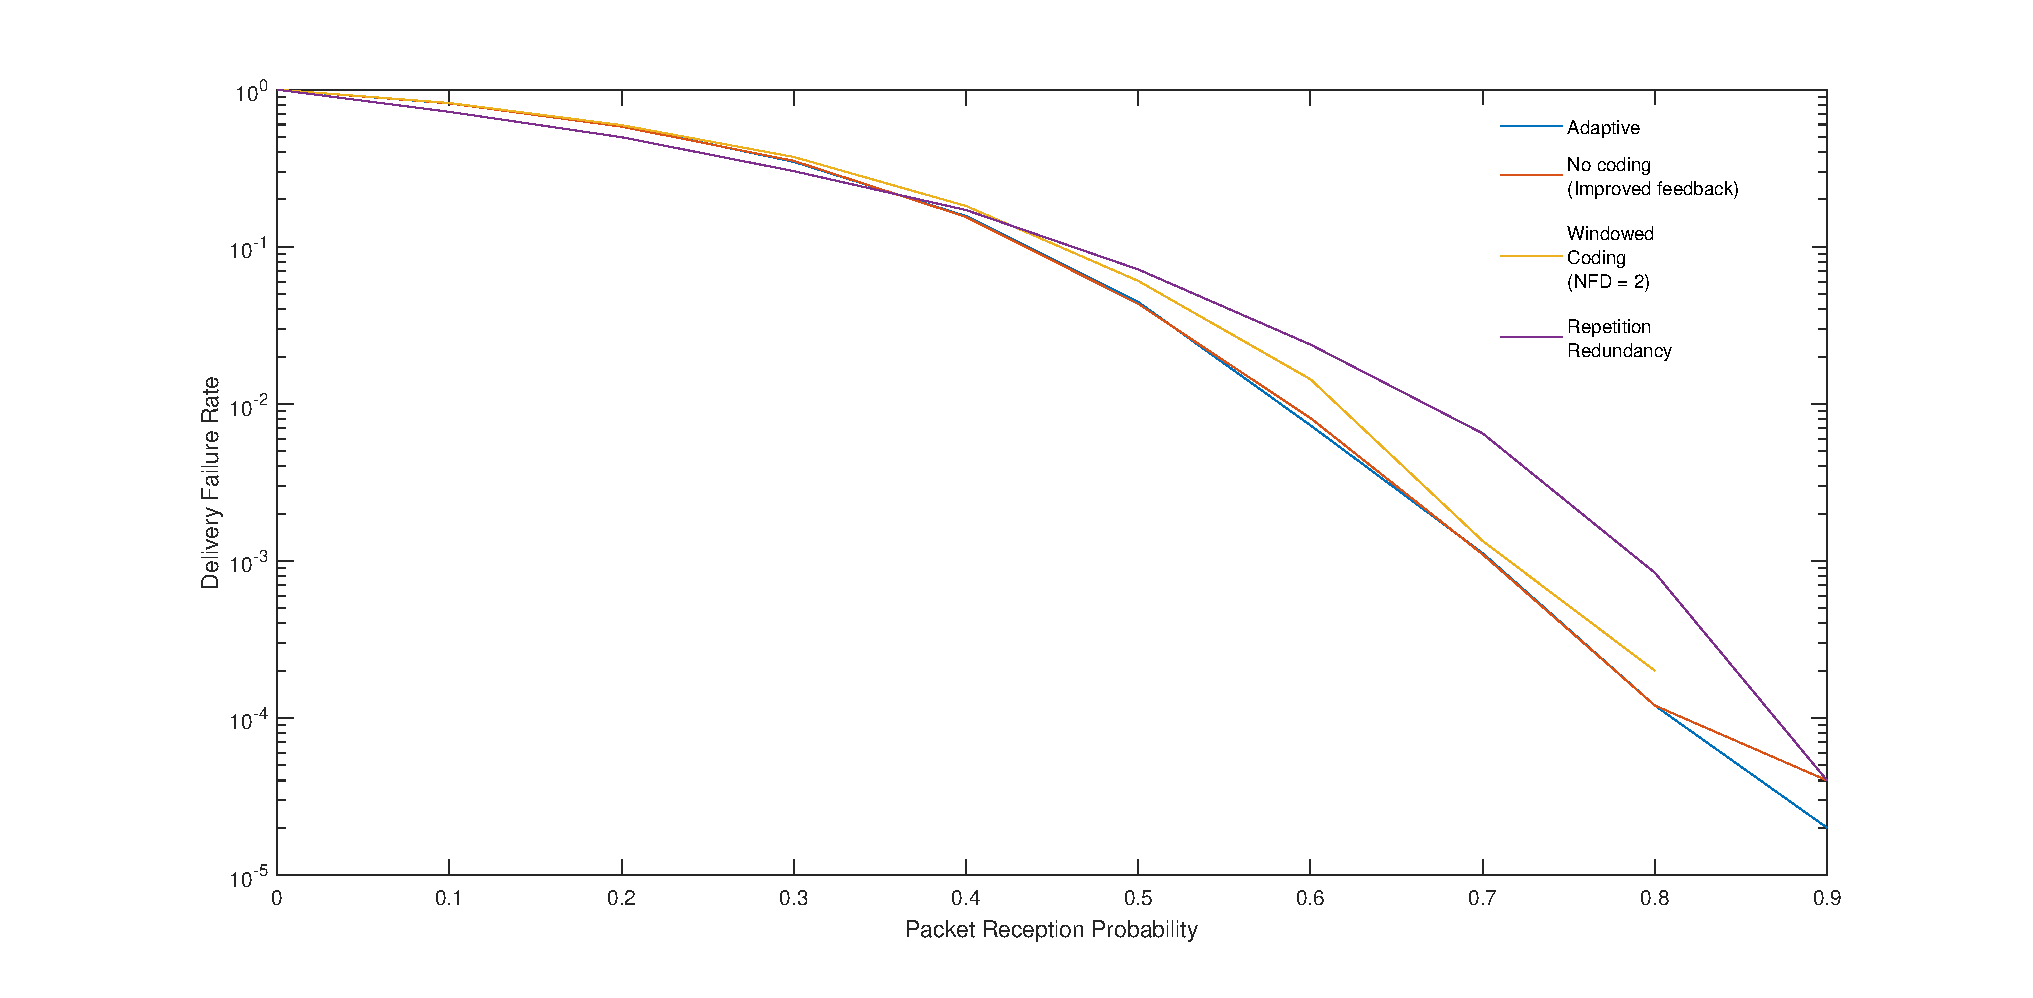
\includegraphics[width=15cm,height=10cm,keepaspectratio]{results-delay=16-feed=4-switch}
	\caption{Similar simulation as in Fig. \ref{results-feed-1} but with $\delta_{max}=16$ i.e $\delta_{max} > l_b$. The no coding performance deteriorates because now most of the missing symbols are outside the range in which it can provide information i.e. in set $[s_{u+l_b+1}, s_i]$.}
	\label{results-feed-2}
\end{figure}

\begin{figure}[t]
	\centering
	\includegraphics[width=15cm,height=10cm,keepaspectratio]{results-delay=16-feed=4-alp=1.5}
	\caption{Similar simulation as in Fig. \ref{results-feed-2} but with $\alpha_0 = 1.5$. The no coding performance is similar to what was before because now also most of the missing symbols are outside the range in which it can provide information i.e. in set $[s_{u+l_b+1}, s_i]$. The adaptive scheme's performance becomes very similar to \textit{windowed coding} because of the transmission take place in the windowed coding mode rather than the improvised feedback mode.\\}
	\label{results-feed-3}
\end{figure}


\subsection{No feedback degree selection}

According to the algorithm of \textit{windowed coding} if feedback for payload $\mathbf{p}_{i-1}$ is not received, then the current payload $\mathbf{p}_{i}$ will contain all coded symbols. The degree of coding is chosen randomly from a uniform distribution between $[1, z]$ where $z = min(i-u_l, i-u_{max})$, $u_l$ is the oldest undelivered sequence in the most recent feedback and $u_{max} = i-\delta_{max}$, the oldest unexpired information symbol at the current instant, $i$. The idea behind this that since no information about the state of symbols is known an assumption is made that all the symbols are equally likely to be missing so a uniform random variable is used to choose the coding degree. But on further thought it is clear that not all symbols have the same probability of missing. The symbols which are older have got more chances in the past to be delivered than recent symbols. In a way the probability of missing should increase for a more recent symbol, but this assumption is only valid if channel erasure is uniform. For Gilbert-Elliot channel where burst errors occur it may be possible that any set of symbols may be lost in a burst and thus no conclusion can be drawn about the missing probability of symbols.

We conduct some experiments with various fixed degrees while coding when no feedback is present. The \textit{Delivery Failure Rate} is quite erratic and sometimes performs even worse than Repetition Redundancy. The best performance is seen when the no feedback coding degree is $2$. There is no clear theoretical understanding why this happens and what should be the optimal no feedback degree for different scenarios. On initial thought, the best performance of $NFD = 2$ can be explained by the decoding process. We know that for successful decoding $d-1$ out of the $d$ combined symbols must already be received. So when the degree is $2$ if anyone among the two is already present decoding is successful but for degree $3$ we would any two of them to be already received and so on for higher degrees. It becomes improbable that atleast $n-1$ symbols are already received for $n$-degree coded symbol as $n$ increases. So most of the transmissions with higher coding degree would not result into a successful deocde and thus the delivery failure rate is higher. 


\begin{figure}[t]
	\centering
	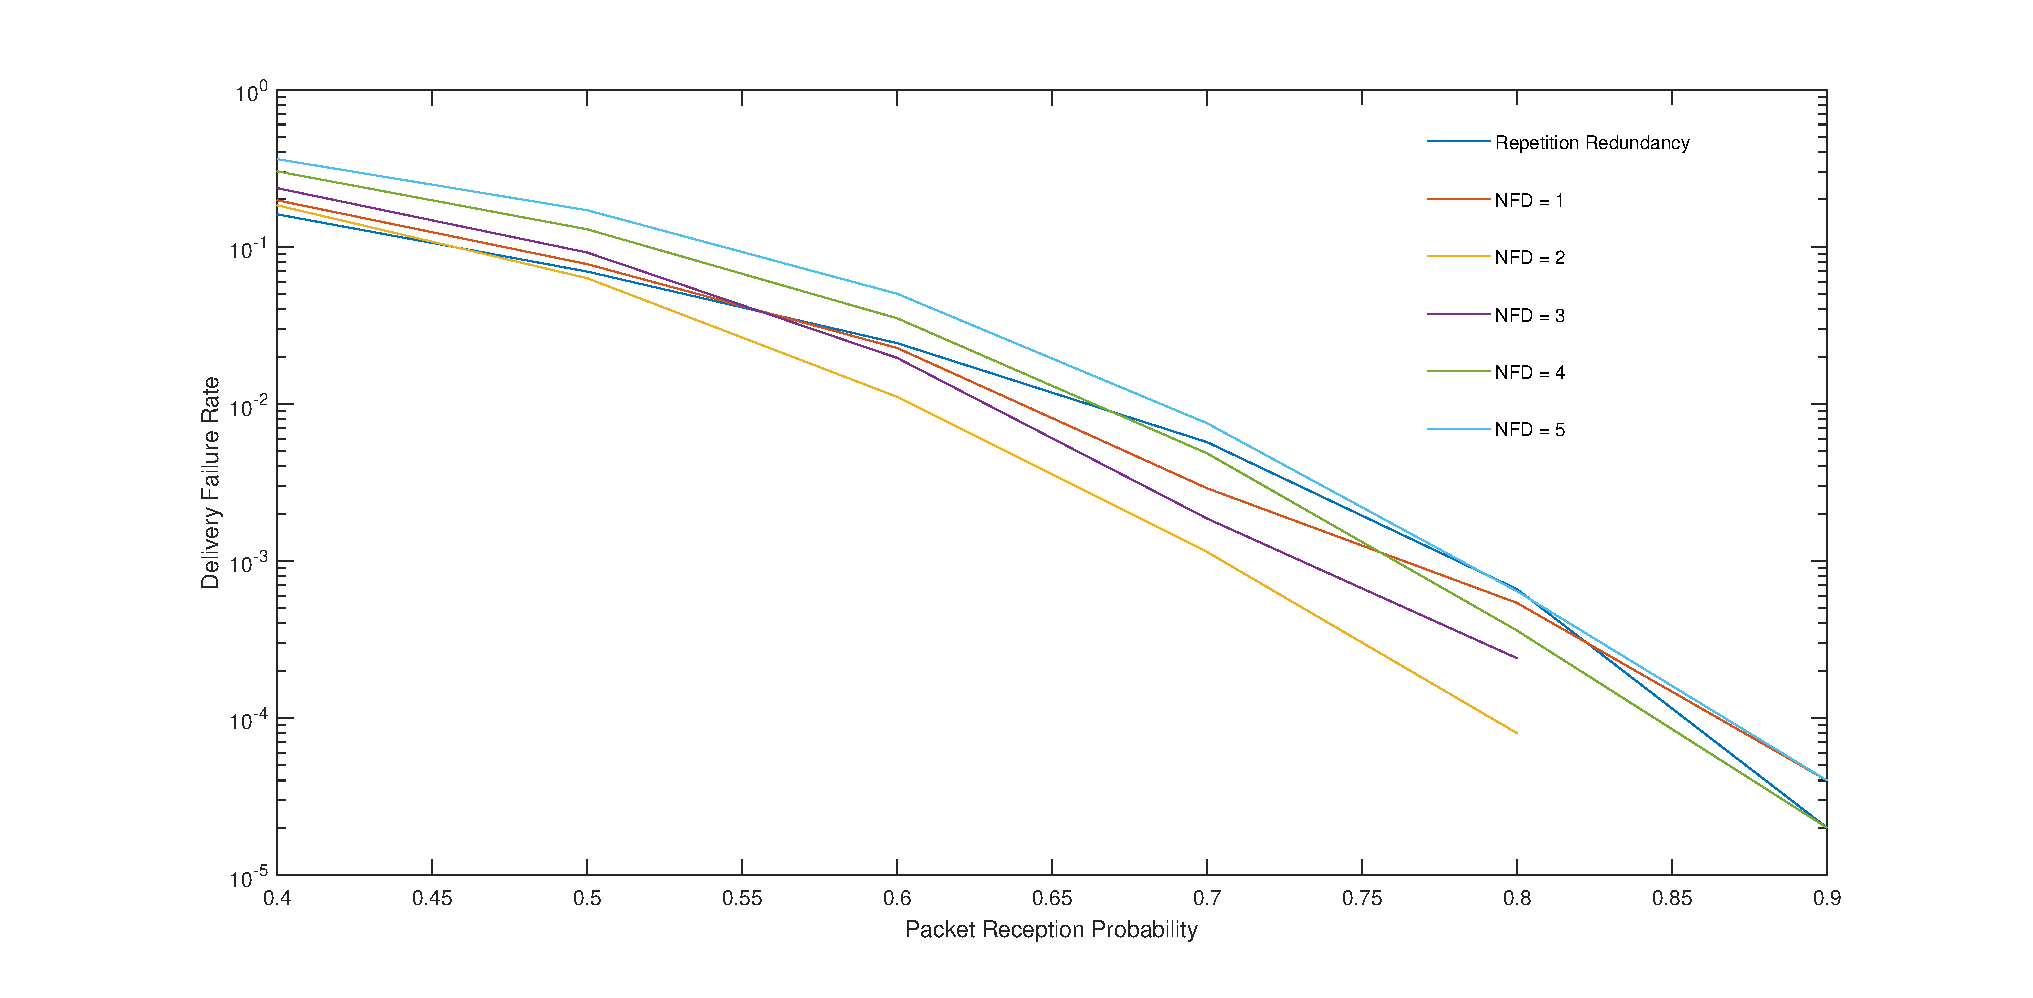
\includegraphics[width=15cm,height=10cm,keepaspectratio]{basic}
	\caption{Delivery Failure Rate v/s Packet Reception Probability with different values of No Feedback Degree (NFD).}
	\label{basic}
\end{figure}


\section{Future Works}
\rhead{Future Works}
In the previous section we have described the analysis that has been completed yet. There are many other things to explore. In coming months our focus will be on the adaptive scheme and how it can be further improved. At the moment, there are some issues with the scheme. Furthermore, there is no theoretical ground to degree selection when there is no feedback. We would explore how to quantify the no feedback state and how to choose optimal degree based on the information which we might have from previous feedback. Even when feedback is present the estimate for optimal degree is suboptimal because when a single payload contains more than one coded symbol joint optimization of degree over both the symbols should be looked into. In this work, the focus has been on the \textit{windowed coding} scheme whereas the paper \cite{borkotokyicc} lists one more algorithm---\textit{selective coding}. \textit{Selective coding} should also be looked into to improve its performance. Apart from all this we also need to evaluate our methods on different channel erasure models as currently we are focusing on Bernouli and Gilbert-Elliot channels. Finally, the role of a buffer at the receiver should also be investigated.



  \newpage
%  %\newpage\null\newpage
  \chapter{Relay}
\label{relay}
\graphicspath{{Chapter_4/Vector/}{Chapter_4/}}

Our analysis in preceding chapters has been limited to the study of single source to gateway point to point communication. In this chapter we introduce a relay node between the source and the gateway and we evaluate the performance gain and constraints in such a setting. 

\section{Basic Relay Operations}
\rhead{Basic Relay Operations}

A relay node in a network is usually tasked with increasing the redundancy and routing the packets generated at the source, when direct transmissions between source and receiver may be hampered or impossible. The sender sends the message packet both to the receiver directly and simultaneously to the relay. Now, if the direct transmission between the source and receiver fails, the relay node may decide to retransmit that packet some time in the future. This leads to the development of an additional redundant path from the source to the receiver. The additional link established is more reliable as the probability of packet loss between source to relay, and, relay to receiver, is smaller than direct source to receiver transmission. This is because the relay is usually placed closer to the source than the receiver is from the source.

\begin{figure}[t]
	\centering
	\includegraphics[width=10cm,height=8cm,keepaspectratio]{relay.png}
	\caption{The additional link established due to relay node.}
	\label{relay-fig}
\end{figure}


\subsection{Relay Baseline}

It is obvious that if we add a relay in any network the net performance in terms of packet delivery will increase due to the additional path and redundancy. So to evaluate our methods (which would describe later) we need to create a relay baseline against which we would compare our results.

First, we describe a few assumptions on the relay node which we introduce in the network:
\begin{itemize}
	\item \textbf{Memory size:} The relay has fixed memory which we describe as the number of maximum source messages it can store. In our case we only keep the uncoded messages which have not yet expired for the relay i.e. in $[s_{i-\delta_{max}}, s_i]$
	\item \textbf{Transmitted packet size:} The relay will transmit a packet which will contain only $1$ message (coded or uncoded). We fix this to $1$ to make sure that energy consumption at the relay can be kept at a minimum.
	\item \textbf{Relay transmission interval:} This is the minimum number of messages which the relay must receive before it can transmit a packet.
	\item \textbf{Packet Success Probability:} It it already known that the channel between the source and relay is more reliable than the channel between source and receiver due to closeness of the relay to the source. But how much reliable? In these experiments we assume that channel between source and relay is two times better than the channel between source and receiver i.e. the packet erasure probability becomes half for the channel between source and relay. Let's assume the packet success probability between source and receiver is $p_s$ then the packet success probability between source and relay will become $1-\frac{1-p_s}{2}$.
\end{itemize} 

We finally define our relay baseline as the normal windowed coding employed at the source and a relay node which does simple forwarding of one message that it receives. The relay waits to receive one packet from the source and once it is received successfully, the relay transmits it to the gateway. We also abstain from coding at the relay node and thus relay transmits only uncoded message. The relay transmission rate for this node is $1$.

\section{Windowed Coding at Relay}
\rhead{Windowed Coding at Relay}
We now employ message coding at the relay intelligently. We create a similar network structure with a source, a relay node and a receiver as in the case of relay baseline. Here both the source and relay node follow the \textit{Windowed Coding} scheme. The relay also receives the feedback from the gateway and since the channel between the relay and gateway is also more reliable the relay receives feedback more frequently as compared to the source.

\subsection{Modifications to Windowed Coding for Relay}

The generic \textit{Windowed Coding} behaves differently when the sender receives a feedback from the receiver and when the feedback is missing. However, the relay does not have all the source symbols in its memory so we can't directly use the nascent Windowed Coding. It may so happen that even if the relay receives a feedback, it may not have required source symbols in its memory to take the desired actions. The general feedback structure as in Fig. \ref{feedback} is used here. The feedback has two important parameters: the \textit{oldest undelivered} symbol, $s_u$ and the \textit{number of missing symbols}, $\beta$ in $[s_u, s_i]$. Based on these values the algorithm decides the degree of coding and choose the symbols to code.

\begin{algorithm}[H]
	\label{window}
	\SetAlgoLined
	\KwResult{Message delivery at the receiver}
	Generate all the messages at the sender\;
	\For{all messages at the sender}{
		\eIf{previous feedback is received}{
			create a packet while choosing a coding degree using the \ref{eq:8};
		}{
			create a packet using the no feedback degree of 2\;
		}
	}
	\caption{Nascent Windowed Coding}
\end{algorithm}


 \begin{algorithm}[H]
 	\label{relay-coding}
 	\SetAlgoLined
 	\KwResult{Message delivery at the receiver}
 	Receive the uncoded messages from the source and store in the memory\;
 	Discard old messages which do not fit in the memory\;
 	\If{number of messages in memory \textbf{greater than equal to} relay transmission interval}{
 		\eIf{previous feedback is received \textbf{and} oldest undelivered message in memory}{
 			create a packet while choosing a coding degree using the \ref{eq:8};
 		}{
 			create a packet using the no feedback degree of 2\;
 		}
 	}
 	\caption{Modified Windowed Coding at Relay}
 \end{algorithm}

 It is quite possible that the relay may not have all the symbols in this range. Suppose the oldest packet which is in relay's memory is $s_{relay}$ such that $s_u$ is older than $s_{relay}$, then is clear that we cannot send $s_u$ directly like we do in nascent \textit{Windowed Coding}. Secondly, the number of missing packets $\beta$ in the interval $[s_u, s_i]$ does not make sense for the interval $[s_{relay}, s_i]$ which is a subset of $[s_u, s_i]$. Thus, the received feedback in this case turns out to be practically useless for the relay to make better decisions. So when this happens we do not utilize the feedback and assume it to be missing and thus create coded packets with degree 2. Finally the relay, sends packets and preform coding following the Algorithm \ref{relay-coding} listed above.
 
\section{Results}
\rhead{Results}

After setting up our system model we simulate it for various values of relay parameters like \textit{'relay memory size'} and \textit{'relay transmission interval'}, we discover some very interesting correlations. In this section we will only discuss the effects of relay parameters as role of other parameters has already been discussed in previous chapters.

\subsection{Delivery Failure Rate}
Delivery Failure Rate (DFR) is the ratio of number of messages undelivered to the total number of messages transmitted. We observe that as we increase the \textit{relay memory size} to a limit (a little higher than $\delta_{max}$) the DFR reduces sharply and the coding scheme performs better than the baseline. For lower values of \textit{memory size} the baseline performs very similar to the relay (coding). Similarly, when the \textit{relay transmission interval} is reduced the DFR reduces owing to higher number of transmissions from the relay. Our goal is to get better performance while keeping the number of relay transmission to a minimum. So, the higher the \textit{relay transmission interval} the more energy efficient is the overall scheme. We get better performance than the baseline for reasonably high \textit{relay transmission interval} but the performance deteriorates for very high values. This trend holds irrespective of the type of channel.

\newpage
% Bernouli
\begin{figure}[H]
	\centering
	\vspace{5ex}
	\begin{subfigure}
		\centering
		\includegraphics[width=15cm,height=10cm,keepaspectratio]{/bernouli/res-m=20-tx=1.png}
		\caption{Delivery Failure Rate v/s Packet Reception for a Bernouli Erasure Channel: The \textit{relay memory size} is $20$ and \textit{relay transmission interval} is $1$. It is evident that even adding a simple relay will improve the performance as shown in the baseline. However, our scheme performs better than a simple forwarding relay.}
		\label{relay-res-1}
	\end{subfigure}

	\vspace{5ex}

	\begin{subfigure}
		\centering
		\includegraphics[width=15cm,height=10cm,keepaspectratio]{/bernouli/res-m=20-tx=10.png}
		\caption{Delivery Failure Rate v/s Packet Reception for Bernouli Erasure Channel:  The \textit{relay memory size} is $20$ and \textit{relay transmission interval} is $10$. Increasing the \textit{relay transmission interval} hampers the performance slightly.}
		\label{relay-res-2}
	\end{subfigure}
\end{figure}

 
% Gilbert
\begin{figure}[H]
	\centering
	\vspace{5ex}
	\begin{subfigure}
		\centering
		\includegraphics[width=15cm,height=10cm,keepaspectratio]{/gilbert/res-dfr-m=20-tx=5.png}
		\caption{Delivery Failure Rate v/s Packet Reception for a Gilbert-Elliot Erasure Channel: The \textit{relay memory size} is $20$ and \textit{relay transmission interval} is $5$. The performance of our method is even better than the Bernouli Channel.}
		\label{relay-res-3}
	\end{subfigure}

	\vspace{5ex}
	
	\begin{subfigure}[b]
		\centering
		\includegraphics[width=15cm,height=10cm,keepaspectratio]{/gilbert/res-dfr-m=20-tx=10.png}
		\caption{Delivery Failure Rate v/s Packet Reception for Gilbert-Elliot Erasure Channel:  The \textit{relay memory size} is $20$ and \textit{relay transmission interval} is $10$.}
		\label{relay-res-4}
	\end{subfigure}
\end{figure}



\subsection{Energy Consumption}

Energy consumption is a vital parameter for any wireless communication network since most of the wireless devices run of a battery so it is critical to ensure we no energy is wasted during transmission. Most of the energy is consumed transmission of a packet and is proportional to the length of the packet.	Every transmission in our design is of fixed packet length so if we count the total number of symbols we transmit we can get an approximate value of the total energy consumed. The total energy consumed for the relay setup would obviously be higher due to the presence of two elements which can transmit so comparing it with the cases when there is no relay will not be fair. Thus, we calculate the average energy consumed per transmitting source by dividing the total energy consumed by $2$. We find that the average energy consumed per transmitting source on introducing the relay is smaller when there was no relay (i.e. only a single source). The extra transmissions made by the relay actually reduce the number of direct transmissions made by the source and thus reduce the average consumed by it too.

\begin{figure}[H]
	\centering
	\includegraphics[width=15cm,height=10cm,keepaspectratio]{/gilbert/res-en-m=20-tx=10.png}
	\caption{Average Energy Consumed v/s Packet Reception for Gilbert-Elliot Erasure Channel:  The \textit{relay memory size} is $20$ and \textit{relay transmission interval} is $10$.}
	\label{relay-res-5}
\end{figure}

\newpage
\section{Summary}
\rhead{Summary}
In this chapter we introduced a relay node in our setup and we found that if we do modified windowed coding at the relay with the symbols available at it we can vast improvements in Delivery Failure Rate and Average Energy Consumption per transmitting source. Introducing a relay in any network improves performance but we demonstrate that our method performs better as compared to introducing a naive relay node in the network.

The goal of this thesis was to improve upon the existing \textit{Windowed Coding Scheme} introduced first in \cite{borkotokyicc}. By the end of it we were able to take substantial steps towards our objective. Finally we introduced a coding scheme or a message transmission protocol which can be utilized in any wireless sensor network to reliably transmit information while being energy and computationally efficient. There are still multiple avenues for improvement namely joint optimization of degree, storing coded messages at relay, buffer at receiver, relay node using the uncoded algorithm, adaptive packet sizes during transmission etc. which are still under our consideration and may help us improve our methods in the future.



 \newpage
 
%\lhead{}
%\rhead{\footnotesize Appendix}
%\appendix
%\addcontentsline{toc}{chapter}{Appendix}
%
%%%%% Creating Appendix A
	\chapter{}
	\label{appendix0}
		\graphicspath{{Appendices/Vector/}{Appendices/}}
	%%% Lauricella's Hypergeometric Functions
	%%%%%
\section*{Title of Appendix}
%%%%%%%%%%%%%%%%%%%%%%%%%%%%%%%%%%% 
%%%%%%%%%%%% Complete System Diagram
%%%%%%%%%%%%%%%%%%%%%%%%%%%%%%%%%%%

xxxxxx xxxxxx xxxxxx xxxxxx xxxxxx xxxxxx xxxxxx xxxxxx xxxxxx xxxxxx xxxxxx xxxxxx xxxxxx xxxxxx xxxxxx xxxxxx xxxxxx xxxxxx xxxxxx xxxxxx xxxxxx xxxxxx xxxxxx xxxxxx xxxxxx xxxxxx xxxxxx xxxxxx xxxxxx xxxxxx xxxxxx xxxxxx xxxxxx xxxxxx xxxxxx xxxxxx xxxxxx xxxxxx xxxxxx xxxxxx xxxxxx xxxxxx xxxxxx xxxxxx.

\begin{align}
y=\alpha\,x+n
\end{align} 
%\input{Appendices/appendix1}
%\input{Appendices/appendix2}
%\input{Appendices/appendix3}
%  \newpage
%  \singlespacing
%%   %\newpage\null\newpage
%\pagestyle{fancy}
%\fancyhf{}
%\rhead{\fancyplain{}{Publications}}
%\cfoot{\fancyplain{}{\thepage}}
%  \addcontentsline{toc}{chapter}{Publications}
%  	\chapter*{Publications}
	\graphicspath{{Publications/Vector/}{Publications/}}
	\noindent{\bf {Journal Publications}}
	\begin{enumerate}
		\item{ }
		\item{ }
		\item{ }
		
		
		
	\end{enumerate}
	\noindent{\bf{Conference Publication}}
	\begin{enumerate}
		\item 
		\item
		
	\end{enumerate}
%  \newpage
\singlespacing
\pagestyle{fancy}
\fancyhf{}
\rhead{\fancyplain{}{Bibliography}}
\cfoot{\fancyplain{}{\thepage}}
\addcontentsline{toc}{chapter}{Bibliography}
\bibliographystyle{IEEEtran}
\bibliography{IEEEabrv,bibliography}


\end{document}

